\documentclass[12pt]{article}       % 設定文件類型為 article,字體大小為 12pt
\usepackage[T1]{fontenc}            % 設定 T1 字型編碼,確保特殊字元的正確顯示
\usepackage{lmodern}                % 強制使用 Latin Modern 字型,提高可讀性和相容性
\usepackage{fontspec}               % 允許使用 OpenType 和 TrueType 字型
\usepackage{graphicx}               % 支援插入圖片
\usepackage{amsmath}                % 提供數學環境和公式支持
\usepackage{csquotes}               % 提供引用格式支援
\usepackage{comment}                % 提供多行註解
\usepackage{ragged2e}
\usepackage{float}

%biber System_Analysis

%=================================================={{{參考文獻設定}}}==================================================

\usepackage[style=ieee, maxnames=99]{biblatex}          % 設定參考文獻格式為 IEEE,最多顯示 99 個作者
\addbibresource{System_Analysis.bib}                       % 添加參考文獻檔案 references.bib
\renewcommand{\bibfont}{\fontspec{Times New Roman}}     % 設定參考文獻字體為 Times New Roman
\renewcommand{\UrlFont}{\fontspec{Times New Roman}}     % 設定 URL 連結字體為 Times New Roman
\DeclareFieldFormat{url}{\url{#1}}                      % 格式化 URL                          % 引用你的 .bib 文件

%=================================================={{{目錄設定}}}==================================================

\usepackage{tocloft} % 自訂目錄格式

% 設定目錄的點線填充樣式
\renewcommand{\cftsecleader}{\cftdotfill{\cftdotsep}}           % 章節(section)
\renewcommand{\cftsubsecleader}{\cftdotfill{\cftdotsep}}        % 小節(subsection)
\renewcommand{\cftsubsubsecleader}{\cftdotfill{\cftdotsep}}     % 子小節(subsubsection)

% 設定圖目錄與表目錄的點線
\renewcommand{\cftdotsep}{1}  % 設定點的間距,使其在所有目錄(含圖、表)中都有效

% 設定目錄標題格式,使目錄、圖目錄、表目錄標題一致
\renewcommand{\contentsname}{\centering \LARGE \textbf{目錄}}    % 目錄標題置中,加粗
\renewcommand{\listfigurename}{\centering \LARGE \textbf{圖目錄}} % 圖目錄標題置中,加粗
\renewcommand{\listtablename}{\centering \LARGE \textbf{表目錄}} % 表目錄標題置中,加粗


%=================================================={{{字體設定}}}==================================================

% 設定英文字體
\newfontface\englishfont{Times New Roman}               % 自訂英文字體命令 \englishfont,使用 Times New Roman

\setmainfont[
    ItalicFont={Times New Roman Italic},                % 設定斜體
    BoldFont={Times New Roman Bold},                    % 設定粗體
    BoldItalicFont={Times New Roman Bold Italic}        % 設定粗斜體
]{Times New Roman}                                      % 設定主要英文字體為 Times New Roman

% 設定中文字體

\usepackage{xeCJK}                                      % 使用 xeCJK 宏包以支援中文
\renewcommand{\figurename}{圖}                           % 設定圖表名稱
\renewcommand{\tablename}{表}                            % 修改表格標題為「表」
\setCJKmainfont[BoldFont={標楷體-繁}, ItalicFont={標楷體-繁}] {標楷體-繁}

%=================================================={{{版面設定}}}==================================================

% 設定頁面邊界,適用 A4 紙張
\usepackage[top=2cm, bottom=2cm, left=2cm, right=2cm, a4paper]{geometry}

% 設定行距與段落格式
\usepackage{setspace}
\onehalfspacing % 設定 1.5 倍行距
\setlength{\parskip}{6pt} % 設定段落間距 6pt
\setlength{\parindent}{2em} % 設定段落首行縮排 2 個字元

%=============================================================================================================================
%=============================================================================================================================
%=============================================================================================================================

\begin{document}
%=================================================={{{封面}}}==================================================
\begin{titlepage}
    \centering
    \vspace*{1cm} % 增加上方間距

    {\LARGE \textbf{元智大學工程學院機械工程學系}} \\[0.5cm] % 標題較大且加粗
    {\LARGE {Department of Mechanical Engineering}} \\[0.5cm] % 標題較大且加粗
    {\LARGE {College of Engineering}} \\[0.5cm]
    {\LARGE {Yuan Ze University}}

    \vfill % 這一行讓前面的資訊靠上排列

    {\LARGE{[自動販賣機機電整合系統] 之功能與系統架構剖析}} % 這行會上下左右完全置中

    \vfill % 這一行讓後面的資訊靠下排列

    {\LARGE {1100826 王子晨}}\\[4.5cm]
    {\LARGE {指導教授:吳昌暉\hspace{0.5cm}博士}}\\[0.5cm]

\end{titlepage}
\newpage
\pagenumbering{roman}  
\setcounter{page}{1}  % 從 I 開始


\begin{center}
    \tableofcontents    % 生成目錄

\end{center}

%=================================================={{{內容開始}}}==================================================
\newpage  % 插入換頁命令,將目錄和後續內容分開
\pagenumbering{arabic}  % 開始使用阿拉伯數字頁碼
\setcounter{page}{1}  % 設定頁碼從 1 開始

%\englishfont{this is an example of mixed English and Chinese.}
\section{\centering 引言}
%==============================摘要內容==============================
\hspace{2em}自動販賣機作為現代零售業的重要組成部分,其提供了無人自助銷售的便利服務。
隨著科技的進步,傳統的自動販賣機逐漸演變為智能販賣機,融合了物聯網、電子支付、人工智慧等技術,提升了用戶體驗和運營效率。
本報告將深入探討自動販賣機的整體功能、機械結構、致動器與感測器配置,以及人機介面的設計,並對其系統架構進行全面剖析。
%==============================摘要內容==============================

\section{\centering 整體功能}
%==============================內文==============================
\hspace{2em}
自動販賣機\cite{csdn_vending_machine_design_2025}的主要功能是提供全天候的自助商品銷售服務,滿足消費者隨時隨地的購物需求。
其核心功能包括:商品展示與選擇、支付處理、商品出貨、庫存管理、故障診斷。
\begin{figure}[H]
    \centering
    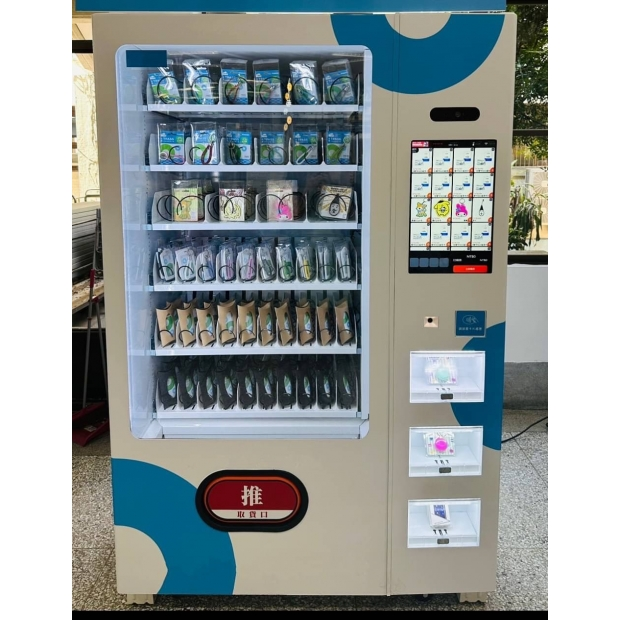
\includegraphics[width=0.7\textwidth]{20231108092414cql0q.jpg}     %圖片檔案名稱
    \caption{自動販賣機\cite{chengli_ticket_machine_2025}}    %圖片檔案名稱
    \label{fig:example2}    %為圖片添加標籤
    %如\ref{fig:example2}所示
\end{figure} 
%==============================內文==============================

\subsection{商品展示與選擇} 
%==============================內文==============================
\hspace{2em}
自動販賣機透過機身上的顯示介面,向消費者展示可供選購的商品資訊。
這些介面通常採用觸控螢幕或按鍵面板,顯示商品的名稱、價格、圖片等詳細資訊。
消費者可以瀏覽商品列表,根據個人需求選擇心儀的商品。
此外,部分先進的自動販賣機還配備語音提示功能,為消費者提供操作指引,提升使用體驗。
%==============================內文==============================

\subsection{支付處理} 
%==============================內文==============================
\hspace{2em}
為了滿足不同消費者的支付習慣,自動販賣機支持多種支付方式,包括現金信用卡、悠遊卡、行動支付(如Apple Pay、Line Pay等),方便消費者完成交易。
支付處理系統的核心是高效、安全的交易流程。當消費者選擇商品並進行支付時,系統會即時驗證支付資訊,確保交易的合法性和安全性。
同時,系統還具備找零功能,當支付金額超過商品價格時,會自動找零給消費者。
%==============================內文==============================

\subsection{商品出貨} 
%==============================內文==============================
\hspace{2em}
在確認支付成功後,自動販賣機啟動商品出貨流程。內部的機械傳動系統將選定的商品從儲存區輸送至取貨口。
常見的商品輸送機構包括傳送帶、螺旋輸送器、推杆等。
為了確保商品順利出貨並防止卡貨,機器內部通常配備光電感測器,實時監測商品的移動狀態。
一旦商品成功到達取貨口,系統會通知消費者取貨。部分自動販賣機還設有防盜設計,確保只有在支付完成後,取貨口才會開啟。
%==============================內文==============================

\subsection{庫存管理} 
%==============================內文==============================
\hspace{2em}
自動販賣機配備先進的庫存管理系統,實時監控每種商品的庫存量。每個商品儲存單元內部裝有感測器,能夠精確計算剩餘的商品數量。
當某種商品的庫存量低於設定的閾值時,系統會自動發出補貨通知,提醒運營人員及時補充貨源。
此外,透過遠端監控技術,運營人員可以隨時查看各地自動販賣機的庫存狀態,進行統一管理和調度,提升運營效率。
%==============================內文==============================

\subsection{故障診斷} 
%==============================內文==============================
\hspace{2em}
為了確保自動販賣機的穩定運行,機器內建自我檢測和故障診斷功能。
系統持續監測各個組件的運行情況,如支付模組、商品輸送機構、感測器等。
一旦發現異常,系統會立即記錄故障資訊,並透過網路將故障報告傳送給維護人員。
這種主動式的故障管理方式,有助於及時發現問題,縮短維修時間,降低停機風險,確保自動販賣機持續為消費者提供高品質的服務。
%==============================內文==============================

\section{\centering 機械結構}
%==============================內文==============================
\hspace{2em}
自動販賣機的機械結構設計直接影響其功能實現和運營效率。主要組成部分包括:外殼、商品儲存區、商品輸送機構、取貨口。
%==============================內文==============================

\subsection{外殼} 
%==============================內文==============================
\hspace{2em}
外殼由金屬或高強度塑料製成,提供堅固的保護,防止外部損壞和盜竊。
此外,外殼還需具備防水、防塵等特性,以適應各種環境下的運行需求。
外殼的設計還考慮到美觀性,通常採用現代化的外觀設計,以吸引消費者的注意。
%==============================內文==============================

\subsection{商品儲存區} 
%==============================內文==============================
\hspace{2em}
商品儲存區是存放各類商品的空間,內部設有多層貨架或旋轉倉。
每個儲存單元對應一種商品,方便管理和補貨。根據商品的特性,儲存區可能需要具備冷藏或加熱功能,以確保商品的品質和安全。
%==============================內文==============================

\subsection{商品輸送機構} 
%==============================內文==============================
\hspace{2em}
商品輸送機構負責將選定的商品從儲存區輸送至取貨口。常見的輸送機構包括傳送帶、推杆、螺旋輸送器等。
其中,螺旋輸送器由螺旋狀的貨道和電機組成(如\ref{fig:example1}所示),當電機運轉時,螺旋貨道旋轉,將商品推送至取貨口。 
此外,為了確保商品輸送的平穩性和可靠性,輸送機構中常使用免維護的軸承技術和拖鏈系統,以降低維護成本並延長設備壽命。
\begin{figure}[H]
    \centering
    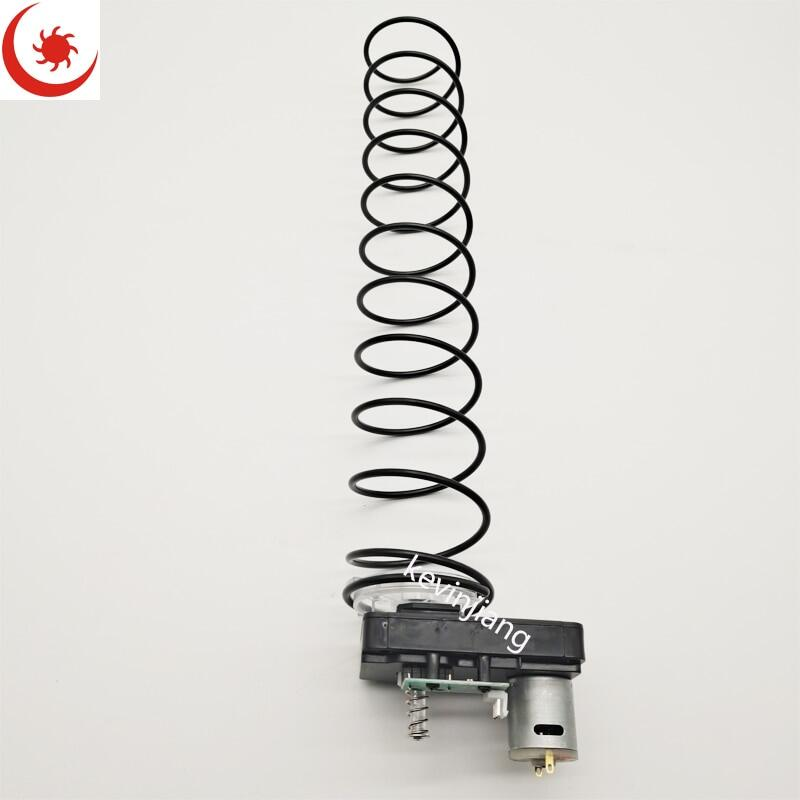
\includegraphics[width=0.7\textwidth]{f33314bafa00371813bbc9cd507c90fb.jpg}     %圖片檔案名稱
    \caption{螺旋輸送器\cite{lazada_vending_machine_2025}}    %圖片檔案名稱
    \label{fig:example1}    %為圖片添加標籤
    %如\ref{fig:example1}所示
\end{figure} 
%==============================內文==============================

\subsection{取貨口} 
%==============================內文==============================
\hspace{2em}
取貨口位於機器前部,消費者可從此處取走購買的商品。通常設有防盜設計,確保只有在支付完成後,取貨口才會開啟。
此外,取貨口的設計還需考慮到防止異物進入和防夾手等安全問題,以保障消費者的使用安全。
%==============================內文==============================

\section{\centering 致動器配置}
%==============================內文==============================
\hspace{2em}
致動器是自動販賣機中執行機械動作的關鍵元件,主要負責商品輸送、取貨口控制等功能。常見的致動器配置如下:直流馬達、步進馬達。
%==============================內文==============================

\subsection{直流馬達} 
%==============================內文==============================
\hspace{2em}
直流馬達主要用於驅動商品輸送機構,如傳送帶、螺旋輸送器等,確保商品順利移動至取貨口。
其運行速度和方向可通過調節電壓和電流進行控制,具有結構簡單、成本較低的優點。
\begin{figure}[H]
    \centering
    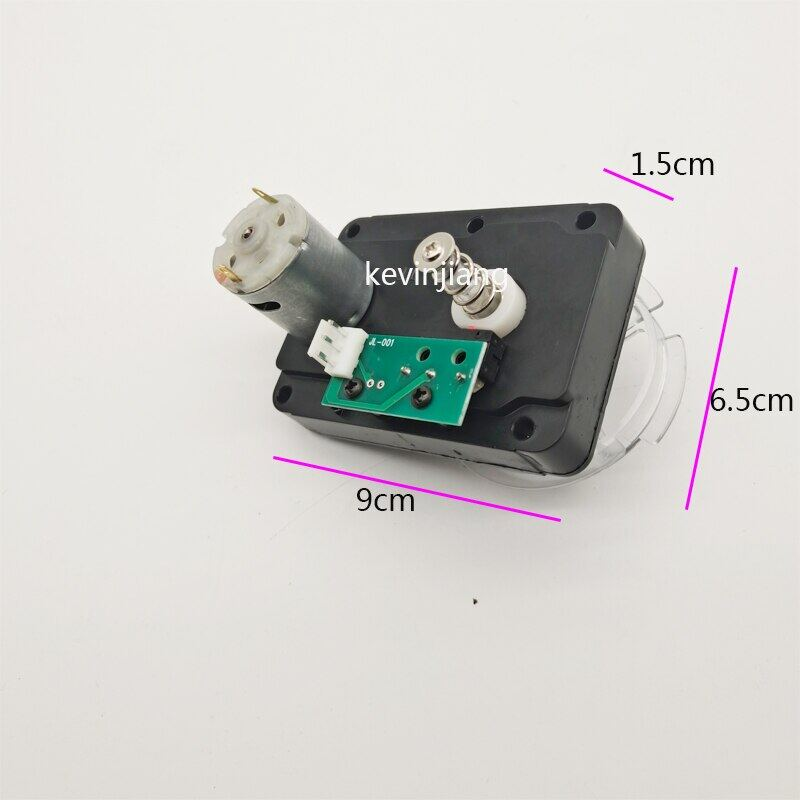
\includegraphics[width=0.7\textwidth]{796df6466ae469d808895d21ce938327.jpg}     %圖片檔案名稱
    \caption{螺旋輸送器馬達\cite{lazada_vending_machine_2025}}    %圖片檔案名稱
    \label{fig:example5}    %為圖片添加標籤
    %如\ref{fig:example1}所示
\end{figure} 
%==============================內文==============================

\section{\centering 感測器配置}
%==============================內文==============================
\hspace{2em}
感測器在自動販賣機中扮演著監測和反饋的角色,確保各項操作的準確性和安全性。
主要的感測器配置包括:光電感測器、硬幣識別器、溫度感測器、庫存感測器
%==============================內文==============================

\subsection{光電感測器} 
%==============================內文==============================
\hspace{2em}
光電感測器利用光束的遮斷或反射來檢測物體的存在與否。
在自動販賣機中,光電感測器被用於檢測商品是否成功掉落至取貨口,防止空投或卡貨情況的發生。
當商品通過感測器的光束時,光束被遮斷,感測器便會發出信號確認商品已成功掉落。
\begin{figure}[H]
    \centering
    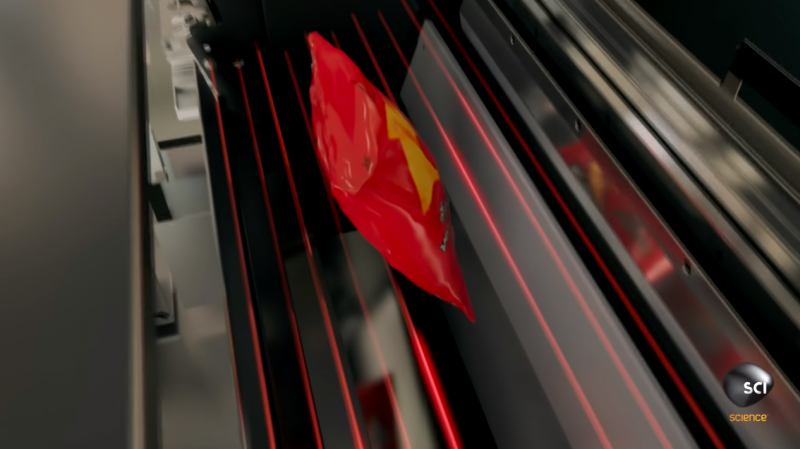
\includegraphics[width=0.7\textwidth]{20181217-113730_U13613_M484183_3853.png}     %圖片檔案名稱
    \caption{光電感測器利\cite{storm_vending_machine_2019}}    %圖片檔案名稱
    \label{fig:example6}    %為圖片添加標籤
    %如\ref{fig:example1}所示
\end{figure} 
%==============================內文==============================

\subsection{硬幣識別器} 
%==============================內文==============================
\hspace{2em}
硬幣識別器如(\ref{fig:example7}所示)是專門用來辨識投入的硬幣的真偽和面額的裝置,確保交易的合法性。
它通常利用感測器檢測硬幣的材質、尺寸、重量等特性,以判斷其真偽和面額。
此外,現代自動販賣機還配備紙幣識別器,用於辨識紙幣的真偽和面額,如\ref{fig:example8}所示。這些識別器的精度和可靠性直接影響交易的成功率和用戶體驗。
\begin{figure}[H]
    \centering
    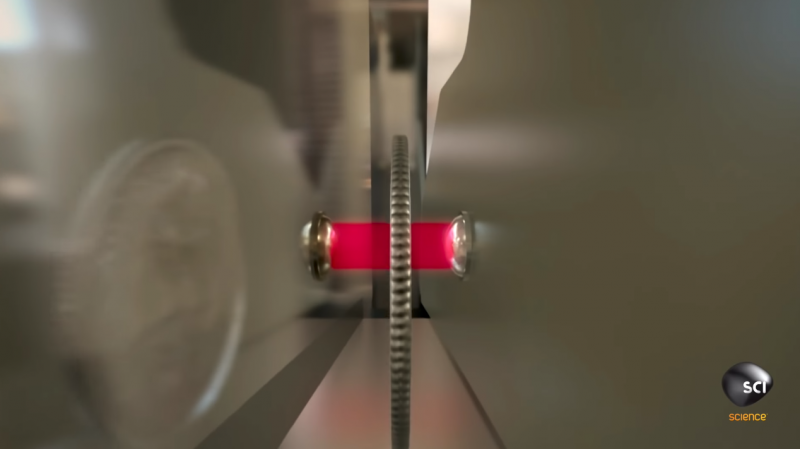
\includegraphics[width=0.7\textwidth]{20181217-113012_U13613_M484168_967b.png}     %圖片檔案名稱
    \caption{利用電磁鐵判斷硬幣材質\cite{storm_vending_machine_2019}}    %圖片檔案名稱
    \label{fig:example7}    %為圖片添加標籤
    %如\ref{fig:example1}所示
\end{figure} 

\begin{figure}[H]
    \centering
    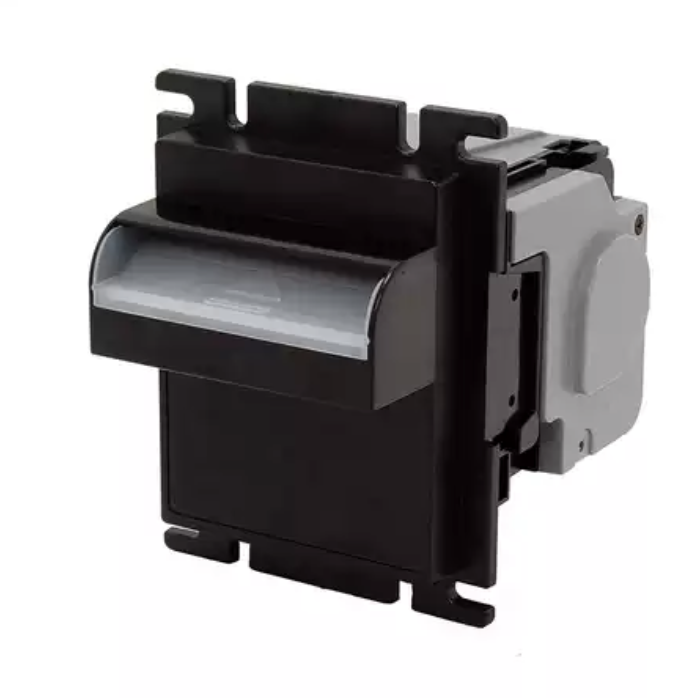
\includegraphics[width=0.7\textwidth]{1234.png}     %圖片檔案名稱
    \caption{紙幣識別器\cite{taobao_product_2025}}    %圖片檔案名稱
    \label{fig:example8}    %為圖片添加標籤
    %如\ref{fig:example8}所示
\end{figure} 
%==============================內文==============================

\subsection{溫度感測器} 
%==============================內文==============================
\hspace{2em}
對於需要冷藏或加熱的商品,自動販賣機內部配備溫度感測器以監測和維持適當的存儲溫度。
溫度感測器能夠實時監測機器內部的溫度變化,確保商品始終處於最佳的存儲環境中,保障商品品質和安全。
%==============================內文==============================

\subsection{庫存感測器} 
%==============================內文==============================
\hspace{2em}
庫存感測器用於監測各商品的剩餘數量,及時發出補貨提醒。常見的庫存感測技術包括重量感測器、光電感測器或RFID技術等。
例如,RFID系統可以實時追蹤商品的進出庫情況,提供精確的庫存資訊,方便管理人員及時補貨。
%==============================內文==============================

\subsection{支付模組} 
%==============================內文==============================
\hspace{2em}
支付模組包含多種支付方式的感測器和讀取器,如信用卡讀取器、NFC感應區等。
這些模組確保自動販賣機能夠支持信用卡、行動支付等多種支付方式,提升消費者的便利性。
支付模組的可靠性和安全性對於交易的成功至關重要,需要定期維護和更新以適應新的支付技術和安全標準。
\begin{figure}[H]
    \centering
    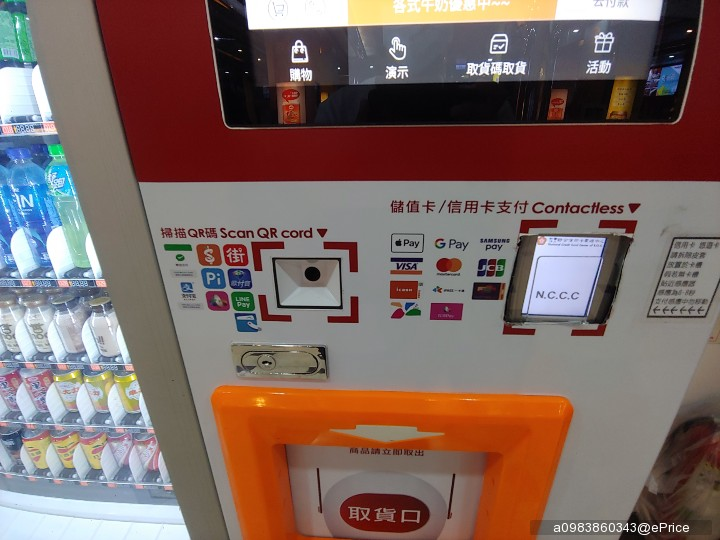
\includegraphics[width=0.7\textwidth]{a0983860343_2_63a7962fecf2018261402695b3dffeef.jpg}     %圖片檔案名稱
    \caption{自動販賣機支付模組\cite{eprice_cashless_vending_machine_2025}}    %圖片檔案名稱
    \label{fig:example3}    %為圖片添加標籤
    %如\ref{fig:example3}所示
\end{figure} 
%==============================內文==============================

\section{\centering 人機介面設計}
%==============================內文==============================
\hspace{2em}
自動販賣機的人機介面是消費者與機器交互的關鍵橋樑,其設計直接影響用戶體驗和操作效率。
一個良好的人機介面應具備直觀、簡潔和多功能的特性,方便各類使用者輕鬆操作。

\subsection{操作介面} 
%==============================內文==============================
\hspace{2em}
自動販賣機的操作介面通常採用觸控螢幕或按鍵面板,主要功能包括商品資訊展示、操作指引與廣告內容。
透過清晰的顯示畫面,消費者能夠輕鬆瀏覽可供選購的商品名稱、價格及庫存狀態,確保選購過程順暢。此外,系統提供明確的操作步驟指引,引導消費者完成選購、支付與取貨的流程,避免因介面不直覺而影響使用體驗。
\begin{figure}[H]
    \centering
    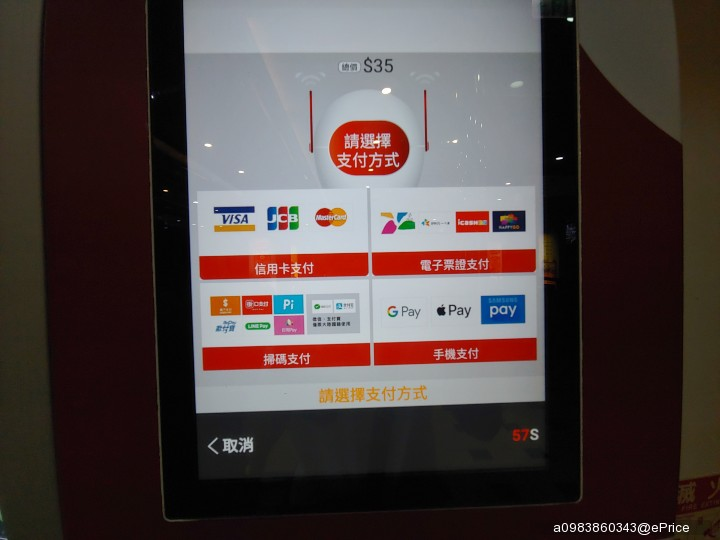
\includegraphics[width=0.7\textwidth]{a0983860343_2_e7743433e8979865768e7468e82e8519.jpg}     %圖片檔案名稱
    \caption{自動販賣機支付介面\cite{eprice_cashless_vending_machine_2025}}    %圖片檔案名稱
    \label{fig:example4}    %為圖片添加標籤
    %如\ref{fig:example3}所示
\end{figure} 
%==============================內文==============================

\section{\centering 參考文獻}
\vspace{-3.5em}  % 減少與上方內容的間距
\renewcommand{\refname}{}  % 去除 "References" 標題
\printbibliography  % 列出參考文獻

\end{document}

%=============================================================================================================================
%=============================================================================================================================
%=============================================================================================================================


\begin{comment}

\section{\centering 緒論}
\subsection{研究問題} 
\subsubsection{違規車輛偵測}
    
    %==============================圖片==============================
\begin{figure}[H]
    \centering
    \includegraphics[width=0.7\textwidth]{截圖 2025-01-24 03.21.17.jpg}     %圖片檔案名稱
    \caption{這是圖片的標題}    %圖片檔案名稱
    \label{fig:example2}    %為圖片添加標籤
    %如\ref{fig:example1}所示
\end{figure}
    
    %==============================數學公式==============================
\begin{align}
    a &= b + c \label{eq:1}
    \\
    d &= e - f \label{eq:2}
    %式label{eq:2}
\end{align}
    
    %==============================表格==============================
\begin{table}[H]
    \caption{MSI GP76 Leopard規格}
    \vspace{12pt} % 增加空格
    \renewcommand{\arraystretch}{1.5} % 調整行距以垂直置中
    \centering
    \begin{tabular}{|c|c|}
        \hline
        \textbf{元件} & \textbf{規格}                 \\ \hline
        中央處理器       & Intel(R) Core(TM) i7-10870H \\ \hline
        記憶體         & DDR4 16GB                   \\ \hline
        硬碟          & 1TB SSD                     \\ \hline
        顯卡          & NVIDIA® GeForce® RTX 3060   \\ \hline
        作業系統        & Ubuntu 18.04                \\ \hline
        電池          & 4-Cell 65 Battery (Whr)     \\ \hline
    \end{tabular}
    \label{tab:MSI GP76 Leopard}
    %(具體規格詳見表\ref{tab:MSI GP76 Leopard})
\end{table}
    
    \end{comment}
        